%\documentclass[11pt, english]{article}
\documentclass{standalone}
%\usepackage[latin1]{inputenc}
\usepackage[T1]{fontenc}
\usepackage[utf8]{inputenc}
%\usepackage[english]{babel}   % S P R A A K


% \usepackage{graphicx}    % postscript graphics
\usepackage{amssymb, amsmath, amsthm, amssymb} % symboler, osv
\usepackage{mathrsfs}
%\usepackage{url}
%\usepackage{thmtools}
%\usepackage{enumerate}  % lister $  
%\usepackage{float}
\usepackage{tikz}
\usetikzlibrary{decorations.pathmorphing}
\usetikzlibrary{calc}
\usetikzlibrary{intersections}
%\usepackage{tikz-3dplot}
%\usepackage{subcaption}
%\usepackage[all]{xy}   % for comm.diagram
%\usepackage{wrapfig} % for float right
%\usepackage{hyperref}
%\usepackage{mystyle} % stilfilen      


\begin{document}

%\begin{figure}
%\begin{center}
  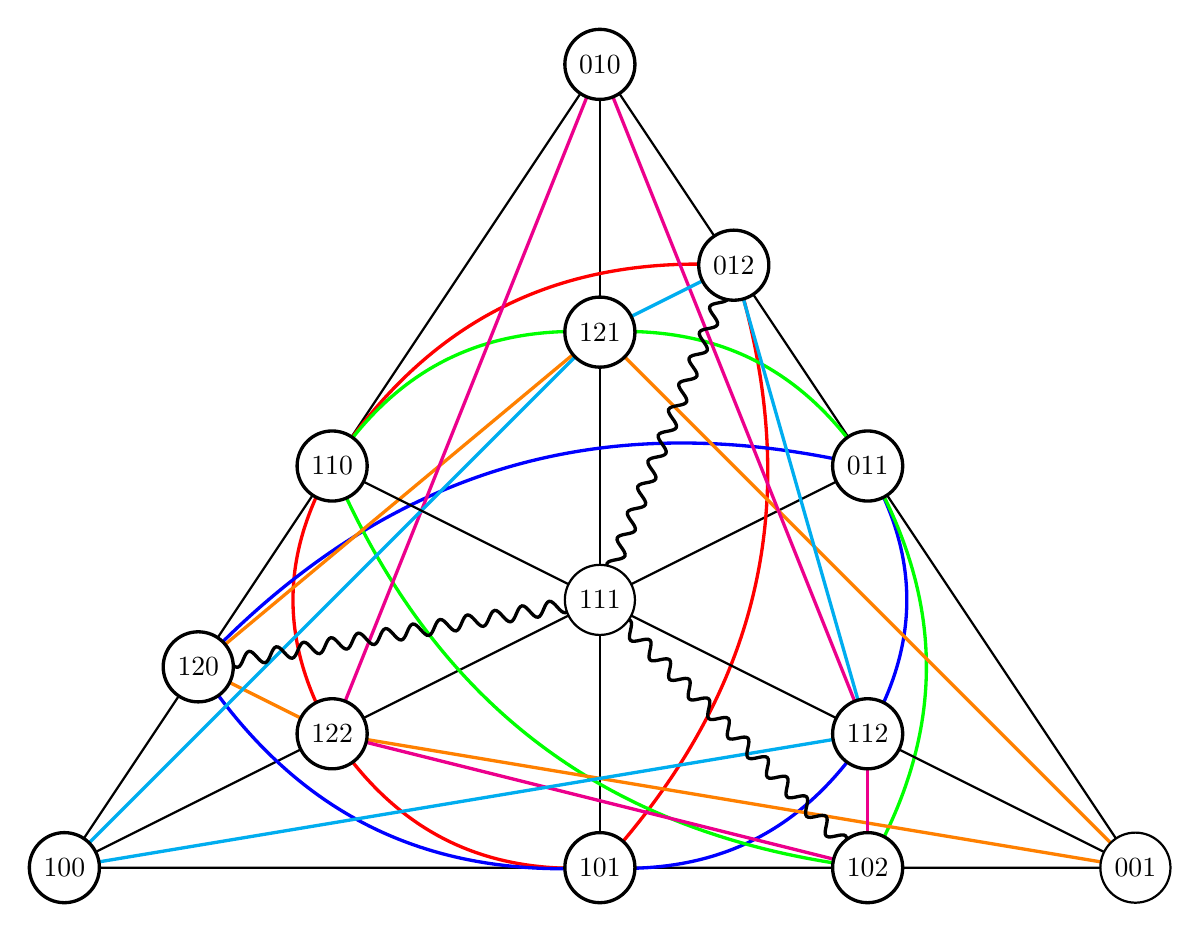
\begin{tikzpicture}[scale=1.7,every node/.style={circle, draw=black, fill=white}, every path/.style={very thick}]
\coordinate (A) at (-4,0);
\coordinate (B) at (4,0);
\coordinate (C) at (0,6);	
\coordinate (D) at (0,0);
\coordinate (E) at (2,0);
\coordinate (F) at (-2,3);
\coordinate (G) at (2,3); % 011
\coordinate (H) at (1,4.5);
\coordinate (I) at (-3,1.5);
\coordinate (J) at (0,2);
\coordinate (K) at (-2,1);
\coordinate (L) at (0,4);
\coordinate (M) at (2,1);

\draw[thick] (A) -- (B)  -- (C) -- cycle;  %1
\draw[thick] (A) -- (K) -- (J) -- (G);   % 2
\draw[thick] (C) -- (L) -- (J) -- (D); % 3
%
\draw[color=red] (D) to[bend left] (K); %1
\draw[color=red] (K) to[bend left] (F);
\draw[color=red] (F) to[bend left] (H);
\draw[color=red] (H) to[bend left] (D);
%
\draw[color=blue] (D) to[bend left] (I); %2
\draw[color=blue] (I) to[bend left] (G);
\draw[color=blue] (G) to[bend left] (M);
\draw[color=blue] (M) to[bend left] (D);
%
\draw[color=green] (E) to[bend left] (F); %3
\draw[color=green] (F) to[bend left] (L);
\draw[color=green] (L) to[bend left] (G);
\draw[color=green] (G) to[bend left] (E);
%
\draw[color=orange] (I) to (L); %5
\draw[color=orange] (L) to (B);
\draw[color=orange] (B) to (K);
\draw[color=orange] (K) to (I);
%
\draw[color=magenta] (C) to (M); %6
\draw[color=magenta] (M) to (E);
\draw[color=magenta] (E) to (K);
\draw[color=magenta] (K) to (C);
%
\draw[color=cyan] (A) to (L); %7
\draw[color=cyan] (L) to (H);
\draw[color=cyan] (H) to (M);
\draw[color=cyan] (M) to (A);
%

\draw[decorate, decoration={snake}] (J) -- (I);
\draw[decorate, decoration={snake}] (J) -- (H);
\draw[decorate, decoration={snake}] (J) -- (E);

\draw[thick] (J) node {111} -- (B) node {001} -- (F); % 11
\draw (A) node {100};
\draw (C) node {010};
\draw (D) node {101};
\draw (E) node {102};
\draw (F) node {110};
\draw (G) node {011};
\draw (H) node {012};
\draw (I) node {120};
\draw (K) node {122};
\draw (L) node {121};
\draw (M) node {112};
\end{tikzpicture}
%\caption{The projective plane $\PP_{\F_3}^2$.}
%\end{center}
%\end{figure}



\end{document}
